\documentclass
%[handout]
{beamer}

%%
%%
%%
% From http://tex.stackexchange.com/questions/2072/beamer-navigation-circles-without-subsections
% Solution #2 or 3:
% \usepackage{etoolbox}
% \makeatletter
% % replace the subsection number test with a test that always returns true
% \patchcmd{\slideentry}{\ifnum#2>0}{\ifnum2>0}{}{\@error{unable to patch}}%
% \makeatother
% Solution #1:
\usepackage{remreset}% tiny package containing just the \@removefromreset command
\makeatletter
\@removefromreset{subsection}{section}
\makeatother
\setcounter{subsection}{1}


\usepackage{etex}
\usepackage{pgf}
\usepackage{tikz}
\usepackage{url}
\usepackage{amsmath}
\usepackage{color}
% \definecolor{red}{rgb}{1,0,0}
\usepackage{ulem}
% \usepackage{booktabs}
\usepackage{colortbl,booktabs}
\renewcommand*{\thefootnote}{\fnsymbol{footnote}}
\usepackage{fancybox}
\usepackage[framemethod=TikZ]{mdframed}
\mdfdefinestyle{FactStyle}{%
  outerlinewidth=0.5,
  roundcorner=1pt,
  leftmargin=1cm,
  linecolor=blue,
  outerlinecolor=blue!70!black,
  backgroundcolor=yellow!40
}
\usepackage{cancel}

  \newcommand\Warning{%
    \makebox[2.4em][c]{%
      \makebox[0pt][c]{\raisebox{.2em}{\Large!}}%
      \makebox[0pt][c]{\color{red}\Huge$\bigtriangleup$}}}%

\usepackage{stackengine}
\usepackage{scalerel}
\usepackage{xcolor}
  \newcommand\dangersign[1][2ex]{%
    \renewcommand\stacktype{L}%
    \scaleto{\stackon[1.3pt]{\color{red}$\triangle$}{\tiny !}}{#1}%
  }



\usepackage{dcolumn}
\newcolumntype{d}[1]{D{.}{.}{#1}}

% From
% http://tex.stackexchange.com/questions/109900/how-can-i-box-multiple-aligned-equations
\usepackage{empheq}
\usepackage{tcolorbox}  \newtcbox{\othermathbox}[1][]{%
  nobeforeafter, tcbox raise base, 
  colback=black!10, colframe=red!30, 
  left=1em, top=0.5em, right=1em, bottom=0.5em}

\newcommand\blue{\color{blue}}
\newcommand\red{\color{red}}
\newcommand\green{\color{green!75!black}}
\newcommand\purple{\color{purple}}
\newcommand\bluegreen{\color{blue!75!green}}
\newcommand\orange{\color{orange}}
\newcommand\redgreen{\color{red!50!green}}
\newcommand\grey{\color{black}}
\newcommand\gap{\vspace{.1in}}
\newcommand\nb{${\red\bullet}\ $}
\newcommand\halfgap{\vspace{.05in}}
\newcommand\divideline{\line(1,0){352}}
\usepackage{marvosym} % for \Smiley

\newcommand{\bluealert}[1]{{\blue\textbf{#1}}}

% \usepackage{beamerthemesplit} %Key package for beamer
\usetheme{Singapore}
% \usetheme{Szeged}
% \usetheme{Garfield}
% \usetheme{CambridgeUS}
% \usenavigationsymbolstemplate{} %Gets rid of slide navigation symbols


\setbeamercolor{separation line}{use=structure,bg=structure.fg!50!bg}
% \begin{beamercolorbox}[colsep=0.5pt]
%   {upper separation line foot}
% \end{beamercolorbox}



\makeatletter
\setbeamertemplate{footline}
{
  \leavevmode%
  \hbox{%
% \begin{beamercolorbox}[colsep=0.5pt]
%   {upper separation line foot}
% \end{beamercolorbox}


  \begin{beamercolorbox}[wd=.5\paperwidth,ht=2.25ex,dp=2ex,colsep=0.5pt]%
    {upper separation line foot}
    \usebeamerfont{author in head/foot}%
    \hspace*{2ex}\insertshortdate:\ \insertshorttitle
  \end{beamercolorbox}%
  \begin{beamercolorbox}[wd=.5\paperwidth,ht=2.25ex,dp=2ex,right]{title in head/foot}%
    \usebeamerfont{title in head/foot}
    {\insertshortauthor}\hspace*{2ex}
  \end{beamercolorbox}}%
  % \begin{beamercolorbox}[wd=.333333\paperwidth,ht=2.25ex,dp=2ex,right]{date in head/foot}%
  %   \usebeamerfont{date in head/foot}\insertshortdate{}\hspace*{2em}
  %   \insertframenumber{} / \inserttotalframenumber\hspace*{2ex} 
  % \end{beamercolorbox}%
  \vskip0pt%
}
\makeatother

\usetikzlibrary{decorations.markings}
\usetikzlibrary{arrows}


\title{Final Exam Review}
\author{Peter Garfield, UCSB Mathematics}
\date{March 15, 2017}
%\institute{}


\useinnertheme{default}

\usefonttheme{serif}
% \usecolortheme{rose}
% \usecolortheme{whale}
% \usecolortheme{orchid}
\usecolortheme{crane}
% \usecolortheme{dolphin}


%TEMPLATE
\setbeamertemplate{navigation symbols}{}

\setbeamertemplate{note page}[compress]

\setbeamertemplate{frametitle}{
  \vspace{0.5em}
  % \begin{centering}
  {\huge\blue\textbf{\textmd{\insertframetitle}}}
  \par
  % \end{centering}
}

% From http://tex.stackexchange.com/questions/7032/good-way-to-make-textcircled-numbers:
\newcommand*\circled[1]{\tikz[baseline=(char.base)]{\node[shape=circle,draw,fill=orange,inner sep=1pt] (char) {#1};}} 
% \renewcommand{\labelenumi}{\circled{\textbf{\arabic{enumi}}}}

\let\olddescription\description
\let\oldenddescription\enddescription
\usepackage{enumitem}
\let\description\olddescription
\let\enddescription\oldenddescription

% \usepackage[loadonly]{enumitem}
\setlist[enumerate,1]{label=\colorbox{orange}{\arabic*.},font=\bfseries}
%\setlist[enumerate,2]{label=\colorbox{blue!25}{(\alph*)},font=\bfseries}
% \setlist[enumerate,1]{label=\arabic*.,font=\bfseries}
\setlist[itemize,1]{label=\red$\bullet$}
\setlist[itemize,2]{label=\blue$\bullet$}

\newcommand\answer[1]{\fbox{#1}}
% \renewcommand\answer[1]{}

\newcommand{\antilog}{\operatorname{antilog}}








\title{Calculus Intro}
\author{Trevor Klar, UCSB Mathematics}
\date{July 25, 2022}



\begin{document}
\small
\renewcommand{\fbox}{}



\frame{
  \frametitle{}
  {\Huge{}Welcome To Math 34A!}\\[.5em]

  {\Huge{}Differential Calculus}
  \vfill
  {\Large{}Instructor:}\\
  \ \hspace*{0.2in} Trevor Klar, \url{trevorklar@math.ucsb.edu}\\
  \ \hspace*{0.2in} South Hall 6431X (Grad Tower, 6th floor, blue side, first door on the right)
  \\[0.5em]

  {\Large{}Office Hours:}\\
  \ \hspace*{0.2in} MTWR after class 2:00-3:00, and by appointment. Details on Gauchospace. 
  \bigskip

  {\tiny \copyright\ 2017-22\ Daryl Cooper, Peter Garfield, Ebrahim Ebrahim, Nathan Schley, and Trevor Klar}\\
  Please do not distribute outside of this course.
  \vfill

}


\section*{Review}


\frame{
  \frametitle{Meanings: The Second Derivative}

  \begin{center}
    \begin{tikzpicture}[x=15mm,y=5mm,>=latex]
      \only<1>{%
        \draw[ultra thick,blue,domain=-1:3,smooth] plot (\x,{(\x)^3-3*(\x)^2+2});
      }
      \only<2->{%
        \draw[ultra thick,green!50!black,domain=-1:1,smooth] plot (\x,{(\x)^3-3*(\x)^2+2});
        \draw[ultra thick,orange!90!black,domain=1:3,smooth] plot (\x,{(\x)^3-3*(\x)^2+2});
        \filldraw[blue] (1,0) circle (2pt);
      }
      \uncover<3->{%
        \draw[ultra thick,green!50!black,<-] (-1,-2.5) -- (1,-2.5);
        \draw[green!50!black,fill=white] (1,-2.5) circle (2pt);
        \draw[ultra thick,orange!90!black,->] (1,-2.85) -- (3,-2.85);
        \draw[orange!90!black,fill=white] (1,-2.85) circle (2pt);
        \node[green!50!black] at (0,-3.5) {$f(x)$ cc down};
        \node[orange!90!black] at (2,-3.5) {$f(x)$\ cc up};
      }
      \begin{scope}
        \clip (-1.5,-4) rectangle (3.5,2.75);
              \uncover<4->{%
        % Tangent lines to $y=x^3-3x^2+2$ has slope $y'=3x^2-6x=3x(x-2)$.
        % \draw[blue,domain=-1:0] plot (\x,{(-5/5)^3-3*(-5/5)^2+2+3*(-5/5)*(-5/5-2)*(\x+5/5)});
        % \draw[blue,domain=-1:0] plot (\x,{(-4/5)^3-3*(-4/5)^2+2+3*(-4/5)*(-4/5-2)*(\x+4/5)});
        % \draw[blue,domain=-1:0] plot (\x,{(-3/5)^3-3*(-3/5)^2+2+3*(-3/5)*(-3/5-2)*(\x+3/5)});
        % \draw[blue,domain=-1:0] plot (\x,{(-2/5)^3-3*(-1/5)^2+2+3*(-2/5)*(-2/5-2)*(\x+2/5)});
        % \draw[blue,domain=-1:0] plot (\x,{(-1/5)^3-3*(-1/5)^2+2+3*(-2/5)*(-1/5-2)*(\x+1/5)});
        % \draw[blue,domain=-1:0] plot (\x,{(-1/3)^3-3*(-1/3)^2+2+3*(-1/3)*(-1/3-2)*(\x+1/3)});
        \draw[thick,green!50!black,domain=-1:0] plot (\x,{(-2/3)^3-3*(-2/3)^2+2+3*(-2/3)*(-2/3-2)*(\x+2/3)});
        \draw[thick,green!50!black,domain=-1:0.3333] plot (\x,{(-1/3)^3-3*(-1/3)^2+2+3*(-1/3)*(-1/3-2)*(\x+1/3)});
        \draw[thick,green!50!black] (-0.5,2) -- (0.5,2);
        \draw[thick,green!50!black,domain=-0.3333:1] plot (\x,{(1/3)^3-3*(1/3)^2+2+3*(1/3)*(1/3-2)*(\x-1/3)});
        \draw[thick,green!50!black,domain=0:1] plot (\x,{(2/3)^3-3*(2/3)^2+2+3*(2/3)*(2/3-2)*(\x-2/3)});
        % \draw[thick,red,domain=0:1.85] plot (\x,{(1)^3-3*(1)^2+2+3*(1)*(1-2)*(\x-1)});
        % \draw[thick,blue,domain=2.2:3.5] plot (\x,{(2.5)^3-3*(2.5)^2+2+3*(2.5)*(2.5-2)*(\x-2.5)});
        \fill[black] ({-2/3},{(-2/3)^3-3*(-2/3)^2+2}) circle (2pt);
        \fill[black] ({-1/3},{(-1/3)^3-3*(-1/3)^2+2}) circle (2pt);
        \fill[black] (0,2) circle (2pt);
        \fill[black] ({1/3},{(1/3)^3-3*(1/3)^2+2}) circle (2pt);
        \fill[black] ({2/3},{(2/3)^3-3*(2/3)^2+2}) circle (2pt);
        % \fill[black] (1,{(1)^3-3*(1)^2+2}) circle (2pt);
        % \fill[black] (2.5,{(2.5)^3-3*(2.5)^2+2}) circle (2pt);
      }
      \uncover<6->{%
        \draw[thick,orange!90!black,domain=2.3:3.3] plot (\x,{(8/3)^3-3*(8/3)^2+2+3*(8/3)*(8/3-2)*(\x-8/3)});
        \draw[thick,orange!90!black,domain=1.9:2.9] plot (\x,{(7/3)^3-3*(7/3)^2+2+3*(7/3)*(7/3-2)*(\x-7/3)});
        \draw[thick,orange!90!black] (1.5,-2) -- (2.5,-2);
        \draw[thick,orange!90!black,domain=1.3333:2.1] plot (\x,{(5/3)^3-3*(5/3)^2+2+3*(5/3)*(5/3-2)*(\x-5/3)});
        \draw[thick,orange!90!black,domain=0.5:2] plot (\x,{(4/3)^3-3*(4/3)^2+2+3*(4/3)*(4/3-2)*(\x-4/3)});
        % \draw[thick,red,domain=0:1.85] plot (\x,{(1)^3-3*(1)^2+2+3*(1)*(1-2)*(\x-1)});
        % \draw[thick,blue,domain=2.2:3.5] plot (\x,{(2.5)^3-3*(2.5)^2+2+3*(2.5)*(2.5-2)*(\x-2.5)});
        \fill[black] ({4/3},{(4/3)^3-3*(4/3)^2+2}) circle (2pt);
        \fill[black] ({5/3},{(5/3)^3-3*(5/3)^2+2}) circle (2pt);
        \fill[black] (2,-2) circle (2pt);
        \fill[black] ({7/3},{(7/3)^3-3*(7/3)^2+2}) circle (2pt);
        \fill[black] ({8/3},{(8/3)^3-3*(8/3)^2+2}) circle (2pt);
      }
      \end{scope}
      \uncover<5->{%
        \node[green!50!black] at (0,-4.5) {$f''(x)<0$};
      }
      \uncover<7->{%
        \node[orange!90!black] at (2,-4.5) {$f''(x)>0$};
      }
    \end{tikzpicture}
  \end{center}
  \vspace*{-1em}

  \uncover<8->{%
    \bluealert{Point:} 

    \begin{mdframed}[style=FactStyle]
      \vspace*{-1.25em}
      \begin{align*}
        {\color{orange!90!black}f''(x) > 0} 
        & \iff\ \text{$f'(x)$\ is increasing} \\
        & \iff\ \text{$f(x)$\ is concave up} \\[0.5em]
        {\color{green!50!black}f''(x) < 0}
        & \iff\ \text{$f'(x)$\ is decreasing} \\
        & \iff\ \text{$f(x)$\ is concave down} 
      \end{align*}
    \end{mdframed}
  }
  \vspace*{3in}

}



\frame{
  \frametitle{Concavity}

  \begin{mdframed}[style=FactStyle]
    \vspace*{-1.25em}
    \begin{align*}
      {\color{orange!90!black}f''(x) > 0} & \iff\ \text{$f(x)$\ is concave up} \\
      {\color{green!50!black}f''(x) < 0} & \iff\ \text{$f(x)$\ is concave down} 
    \end{align*}
  \end{mdframed}

  {\red(1)}\ For which values of $x$ is $f(x)=x^3-6x^2+3x+2$ concave up?
  \begin{center}
    A\ when $x=0$
    \quad 
    B\ when $x<6$
    \quad 
    C\ when $x>6$\\
    \ 
    \quad 
    D\ when $x<2$
    \quad 
    E\ when $x>2$
    \quad
    \uncover<2->{\fbox{E}}
  \end{center}

  \uncover<3->{
  {\red(2)}\ Where is $f{\red''}(x)>0$? 

  \
  \hfill
  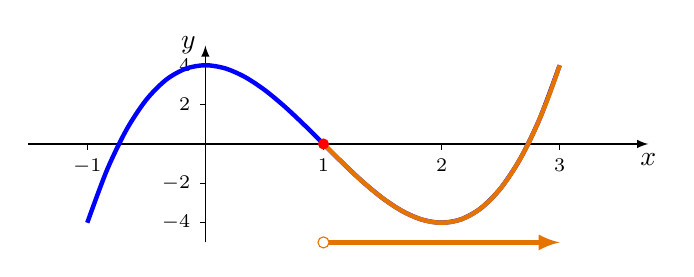
\begin{tikzpicture}[x=15mm,y=2.5mm,>=latex]
    %
    \draw[thin,black,->] (-1.5,0) -- (3.75,0) node[below] {$x$};
    \draw[thin,black,->] (0,-5) -- (0,5) node[left] {$y$};
    % ticks:
    \foreach \x in {-1,1,2,3}
    {
      \draw[thin,black] (\x,0) -- (\x,-2pt) node[below] {$\scriptstyle\x$};
    }
    \foreach \y in {-4,-2,2,4}
    {
      \draw[thin,black] (0,\y) -- (-2pt,\y) node[left] {$\scriptstyle\y$};
    }
    \draw[ultra thick,blue,domain=-1:3,smooth] plot (\x,{2*(\x)^3-6*(\x)^2+4});
    \uncover<4->{%
      \draw[ultra thick,orange!90!black,domain=1:3,smooth] plot (\x,{2*(\x)^3-6*(\x)^2+4});
      \draw[ultra thick,orange!90!black,->] (1,-5) -- (3,-5);
      \draw[orange!90!black,fill=white] (1,-5) circle (2pt);
      \fill[red] (1,0) circle (2pt);
    }
  \end{tikzpicture}
  \hfill
  \ 
  \vspace*{-1em}

  \begin{center}
    A\ when $x<2$
    \quad 
    B\ when $x>2$
    \quad
    C\ when $x<1$\\
    \ 
    \quad 
    D\ when $x>1$
    \quad
    E\ when $-0.7<x<1$
    \pause
    \quad
    \uncover<4->{\fbox{D}}
  \end{center}
}

}


\section{Max / Min Review}

\frame{
  \frametitle{\S8.13: Max/Min problems}

  Often want to find the biggest, smallest, most, least, maximum, minimum of something.

  \begin{minipage}{0.4\linewidth}
    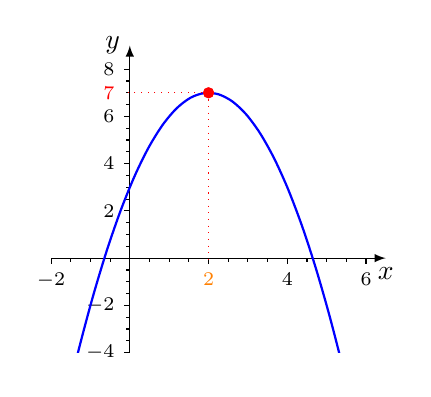
\begin{tikzpicture}[x=5mm,y=3mm,>=latex]
      \draw[thin,black,->] (-2,0) -- (6.5,0) node[below] {$x$};
      \draw[thin,black,->] (0,-4) -- (0,9) node[left] {$y$};
      % ticks:
      \foreach \x in {-2,2,4,6}
      {
        \draw[thin,black] (\x,0) -- (\x,-2pt) node[below] {$\scriptstyle\x$};
      }
      \foreach \x in {-2,-1.5,...,6.2}
      {
        \draw[thin,black] (\x,0) -- (\x,-1.5pt);
      }
      \foreach \y in {-4,-2,2,4,6,8}
      {
        \draw[thin,black] (0,\y) -- (-2pt,\y) node[left] {$\scriptstyle\y$};
      }
      \foreach \y in {-4,-3.5,...,8.2}
      {
        \draw[thin,black] (0,\y) -- (-1.5pt,\y);
      }
      \begin{scope}
        \clip (-2,-4) rectangle (6,8);
        \draw[thick,blue,domain=-2:6.5,smooth] plot (\x,{-1*(\x)^2+4*\x+3});
      \end{scope}
      \uncover<2->{%
        \draw[thin,red,dotted] (2,7) -- (-2pt,7) node[left] {$\scriptstyle7$};
        \fill[red] (2,7) circle (2pt);
      }
      \uncover<3->{%
        \draw[thin,red,dotted] (2,7) -- (2,-2pt) node[below,orange,fill=white] {$\scriptstyle2$};
        \fill[red] (2,7) circle (2pt);
      }
    \end{tikzpicture}
  \end{minipage}
  \hspace*{0.25in}
  \parbox{50mm}{%
    Here's the graph of \\
    $y = f(x)=-x^2+4x+3$
    \gap

    \uncover<2->{%
      The \emph{maximum value} or just \emph{maximum} of the function is ${\red 7}.$ 
    }
    \gap

    \uncover<3->{
      The \emph{value of $x$}\ which gives the maximum of $f(x)$ is $x={\orange 2}$
    }
    \gap

    \uncover<4->{%
      We write ${\blue f({\orange 2})} = {\red 7}$.
    }
  }
  \gap

  \uncover<5->{%
    For this example you can see this is the maximum because
    \begin{equation*}
      f(x) 
      = -x^2+4x+3
      = -(x-{\orange 2})^2+{\red 7}
    \end{equation*}
    $(x-{\orange 2})^2$ is always positive except when $x=\orange 2$\\
    {\blue so the maximum  must} be at $x=\orange 2$.
  }

}

\frame{
  \frametitle{How To Find A Max / Min}

  \begin{mdframed}[style=FactStyle]
    \begin{itemize}
    \item[{\red(1)}] Find $f{\red '}(x)$

    \item[{\red(2)}] Solve $f{\red '}(x)=0.$ This is the $x$ value
      that gives the max / min. 

    \item[{\red(3)}] To find the maximum / minimum plug the value of $x$ found
      in {\red(2)}\ back into $f(x)$. 

    \end{itemize}
  \end{mdframed}
  \vspace*{0.5in}
  \pause

  \alert{Example:}\ Use this method to find the $x$-value where
  \emph{maximum}\ of the function $f(x)=5x-e^{2x}$ occurs.
  \begin{center}
    A $=0$
    \quad 
    B $= \ln(5)$
    \quad 
    C $= 2\ln(5)$
    \quad 
    D $= 2\ln(5/2)$
    \quad 
    E $= \ln(5/2)/2$
    \pause
  \end{center}
  \alert{Answer:}\ \answer{E}
  \vspace*{1in}


}




\section{Word Problems from Last Time}

\frame{ 
  \frametitle{Word Problem \#1} 

  A ball is thrown into the air. After $t$ seconds the height in
  meters above the ground of the ball is $h(t)=40t-10t^2$. How many
  meters high did the ball go?

  \begin{center}
    A $=2$
    \quad 
    B $= 40-20t$
    \quad 
    C $= 20$
    \quad 
    D $= 40$
    \pause
    \quad
    \fbox{D}
  \end{center}
  \vspace*{2in}

}


\frame{
  \frametitle{Word Problem \#2}

  If an airline sells tickets at a price of $\$200+5x$ each the
  number of tickets it sells is $1000-20x$.  What price should the
  tickets be if the airline wants to get the most money?

  \begin{center}
    A $=5$
    \quad 
    B $= 25$
    \quad 
    C $=175$
    \quad 
    D $= 200$
    \quad 
    E $= 225$
    \pause
    \quad
    \fbox{E}
  \end{center}
  \vspace*{2in}

}





\section{Word Problems}

\frame{ 
  \frametitle{Word Problem \#3} 

  A fenced garden with an area of $100\ \text{m}^2$  will be made in
  the shape of a rectangle. It will be surrounded on all four sides by
  a fence. What length and width should be used so the least amount of
  fence is needed? 
  \bigskip
  \pause

  \alert{Approach:}
  \begin{itemize}
  \item[{\blue(1)}] Express the total length of fence in terms of
    \emph{only}\ one variable, either $L = $ length of field, or $W =$
    width of field. This gives a formula for $P=$ (total length of
    fence) involving, say, $W$.
    \pause
    \smallskip

  \item[{\blue(2)}] Find minimum by solving $\dfrac{dP}{dW}=0$.
  \end{itemize}
  \pause
  \bigskip

  Students always find {\blue(1)}\ the hardest part.

  \alert{You}\ have been prepared for this by word problems from chapter 3!
 
  

}



\frame{
  \frametitle{Word Problem \#4}

  A fenced garden with an area of $1000\ \text{m}^2$  will be made in
  the shape of a rectangle. It will be surrounded on all four sides by
  a fence. Three sides are wood fence, and the remaining side is a
  brick wall.
  \begin{itemize}
  \item The wood fence costs \$5 per meter length.
  \item The brick wall costs \$20 per meter length.
    \pause
  \item $C=$ total cost of the fence and brick wall
  \item $L=$ length of the brick wall
  \item $W=$ width of the other side 
  \end{itemize}
  \begin{enumerate}
  \item[\colorbox{blue!50}{(a)}] Find a formula for $C$ in terms of only $L$.
    \vspace*{-0.5em}

    \begin{center}
      A $= 2W + 2L$
      \quad 
      B $= 2000L^{-1}+2L$
      \quad 
      C $= 25L +10000L^{-1}$\\[0.5em] 
      % 
      \ \quad
      D $= 20L + 10000WL^{-1}$
      \quad 
      E $= 5L + 3000$
      \pause
      \quad
      \answer{C}
    \end{center}
    % \bigskip

  \item[\colorbox{blue!50}{(b)}]
    What length of brick wall gives lowest cost?
    \vspace*{-0.5em}

    \begin{center}
      A $= 20$
      \quad 
      B $= 40$
      \quad 
      C $= 50$
      \quad 
      D $= 100$
      \quad 
      E $= 25$
      \pause
      \quad
      \answer{A}
    \end{center}
  \end{enumerate}

}





\frame{ 
  \frametitle{Word Problem \#5} 

  A rectangular field is surrounded by fence. It is divided into 4
  equal
  \begin{center}
    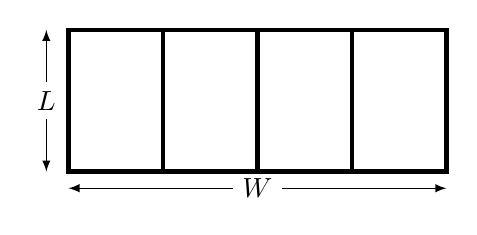
\begin{tikzpicture}[x=12mm,y=6mm,>=latex]
      \draw[thin,black,<->]  (-8pt,0) -- (-8pt,3) node[midway,fill=white] {$L$};
      \draw[thin,black,<->]  (0,-6pt) -- (4,-6pt) node[midway,fill=white] {$W$};
      \draw[ultra thick,black] (1,0) -- (1,3);
      \draw[ultra thick,black] (2,0) -- (2,3);
      \draw[ultra thick,black] (3,0) -- (3,3);
      \draw[ultra thick,black] (0,0) rectangle (4,3);
    \end{tikzpicture}
  \end{center}
  parts by 3 more dividing fences all parallel to one side of the
  field.
  \bigskip

  \begin{enumerate}
  \item[\colorbox{blue!50}{(a)}]\ 
    What is the total length of all the fence needed?
    \begin{center}
      A $= 2L+2W$
      \quad 
      B $= LW$
      \quad
      C $= 5LW$ \\[0.5em]
      \ 
      \quad \quad \quad 
      D $= L+W$
      \quad
      E $= 5L+2W$
      \pause
      \quad \quad \quad 
      \fbox{E}
    \end{center}
    \vspace*{-0.5em}

  \item[\colorbox{blue!50}{(b)}]\ 
    The field must have an area of $1000\ \text{m}^2$.
    Express $W$ in terms of $L$. 
    \begin{center}
      A\ $1000-L$
      \quad 
      B\ $1000L$
      \quad 
      C\ $1000/L$
      \quad 
      D\ $1000+L$
      \pause
      \quad
      \fbox{C}
    \end{center}
  \end{enumerate}
  % \vspace{2in}

}

\frame{ 
  \frametitle{Word Problem \#5 (cont'd)}

  A rectangular field is surrounded by fence. It is divided into 4
  equal
  \begin{center}
    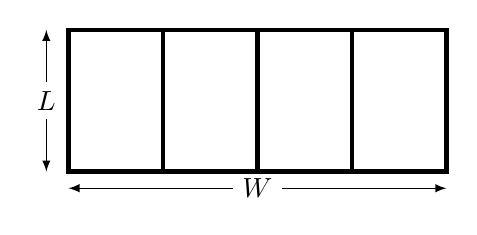
\begin{tikzpicture}[x=12mm,y=6mm,>=latex]
      \draw[thin,black,<->]  (-8pt,0) -- (-8pt,3) node[midway,fill=white] {$L$};
      \draw[thin,black,<->]  (0,-6pt) -- (4,-6pt) node[midway,fill=white] {$W$};
      \draw[ultra thick,black] (1,0) -- (1,3);
      \draw[ultra thick,black] (2,0) -- (2,3);
      \draw[ultra thick,black] (3,0) -- (3,3);
      \draw[ultra thick,black] (0,0) rectangle (4,3);
    \end{tikzpicture}
  \end{center}
  parts by 3 more dividing fences all parallel to one side of the
  field.
  \bigskip

  \begin{enumerate}
  \item[\colorbox{blue!50}{(c)}]\ 
    Express the total length of all the fence needed in terms of $L$.
    \begin{center}
      A $= 5L+1000$
      \quad 
      B $=  5L + 2000/L$
      \quad 
      C $= 5L+2/L$
      \quad
      \pause
      \fbox{B}
    \end{center}

  \item[\colorbox{blue!50}{(d)}]\ 
    What should $L$  be so that the total length of fence used is a minimum?
    \begin{center}
      A $=10$
      \quad 
      B $=20$
      \quad 
      C $= 40$
      \quad 
      D $= 50$
      \pause
      \quad\fbox{B}
    \end{center}
  \end{enumerate}
  \vspace*{2in}
}


\frame{
  \frametitle{Word Problem \#6}

  A rectangular field is surrounded on three sides by a fence and the
  fourth side runs along a perfectly straight river.
  What is the largest area field which can be so enclosed with $120$ meters of fence?
  \begin{center}
    A  $= 1200\ \text{m}^2$
    \quad 
    B  $= 1500\ \text{m}^2$
    \quad 
    C  $= 1800\ \text{m}^2$
    \quad 
    D  $= 1000\ \text{m}^2$
    \quad
    \uncover<3->{%
      \fbox{C}
    }
  \end{center}
  \uncover<2->{%
    \begin{center}
      % \includegraphics[scale=0.5]{fieldriver.pdf}f
      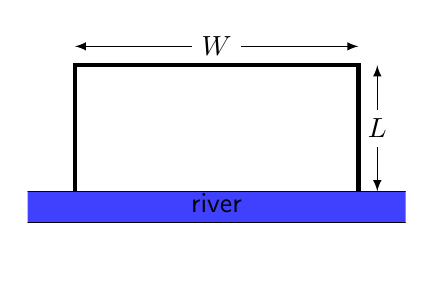
\begin{tikzpicture}[x=12mm,y=8mm,>=latex]
        \draw[thin,black,<->] (0,2.3) -- (3,2.3) node[midway,fill=white] {$W$};
        \draw[thin,black,<->] (3.2,0) -- (3.2,2) node[midway,fill=white] {$L$};
        \draw[ultra thick,black] (0,0) -- (0,2) -- (3,2) -- (3,0);
        \begin{scope}
          \clip (-0.5,0.5) rectangle (3.5,-1);
          \draw[thin,black,fill=blue!75] (-1,0) rectangle (4,-0.5);
          \node[above] at (1.5,-0.5) {\textsf{river}};
        \end{scope}
      \end{tikzpicture}
    \end{center}
  }
}


\frame{
  \frametitle{Word Problem \#7}

  Tickets are going to be sold for a concert.
  \begin{itemize}
  \item If the price of each  ticket is \$40, then $2,000$ tickets
    will be sold. 

  \item For every \$1 the price is decreased, $100$ more tickets will
    be sold.  
  \end{itemize}

  \begin{enumerate}
  \item[\colorbox{blue!50}{(a)}]\ 
    If the tickets are sold for $\$x$ each, how many will be sold?
    \vspace*{-0.5em}

    \begin{center}
      A $=2000-x$
      \quad 
      B $= 2000-100x$
      \quad 
      C $= 2000+100x$\\[0.5em]
      \ \quad\quad\quad
      D $= 6000-100x$
      \quad 
      E $=6000+100x$
      \pause
      \quad\quad\quad
      \fbox{D}
    \end{center}
    \vspace*{-0.5em}
    % \medskip

  \item[\colorbox{blue!50}{(b)}]\ 
    What is the total amount of money generated from selling tickets
    for $\$x$ each? 
    \vspace*{-0.5em}

    \begin{center}
      A $=6000x-100x^2$
      \quad 
      B $= 2000x$
      \\[0.5em]
      \ 
      \quad 
      C $= 2000-40x^2$
      \quad 
      D $=  6000-100x$
      \pause
      \quad
      \fbox{A}
    \end{center}
    \vspace*{-0.5em}
    % \medskip

  \item[\colorbox{blue!50}{(c)}]\ 
    What price should the tickets be to generate the most money from
    sales? 
    \vspace*{-0.5em}

    \begin{center}
      A $=\$20$
      \quad 
      B $= \$22$
      \quad 
      C $= \$24$
      \quad 
      D $= \$30$
      \quad 
      E $= \$40$
      \pause
      \quad
      \fbox{D}
    \end{center}
    % \bigskip
  \end{enumerate}

}



\frame{
  \frametitle{Word Problem \#8}
  
  A farmer is growing wheat.
  \begin{itemize}
  \item On July 1, she has $1,000$ bushels and this increases by $50$
    bushels per day. 

  \item The price of a bushel on July 1 is $\$10$ and is dropping at a rate of $20$ cents per day. 

  \item She will harvest and sell on the same day. 
  \end{itemize}
  How many days should she wait, assuming these trends continue?
  \begin{center}
    A $= 5$
    \quad 
    B $= 10$
    \quad 
    C $= 15$
    \quad 
    D $= 20$
    \quad 
    E $= \text{other}$
    \pause
    \quad
    \fbox{}
  \end{center}
  \vspace*{2in}

}




\end{document}


